\documentclass[11pt]{ltjsarticle}
% タイトルと名前
\newcommand{\mytitle}{タイトル}
\newcommand{\myname}{名前}
% 数式
\usepackage{amsmath,amssymb}
\usepackage{mathtools}
\usepackage{empheq}
\usepackage{amsthm}
\newtheorem{definition}{定義}
\newtheorem{theorem}{定理}
\newtheorem{prf}{証明}
\newtheorem{law}{法則}
\newtheorem{example}{例}
\newtheorem{lemma}{補題}
% 斜体を解除
\makeatletter
\def\th@plain{\upshape}
\makeatother
% 数式フォント
\usepackage{newtxmath}
% フォントの設定
\usepackage{luatexja-fontspec}
\usepackage[haranoaji,no-math,deluxe]{luatexja-preset}
\setmainfont{Times New Roman}
\setsansfont{Source Sans Pro}[
    FontFace = {l}{n}{SourceSansPro-Light}
]
\setmonofont{Source Code Pro}[Scale = 0.875]
% マージンの設定
\usepackage[left=20truemm,right=20truemm,top=25truemm,bottom=30truemm]{geometry}
% 画像関連
\usepackage{graphicx}
% 図を現在位置に挿入
\usepackage{here}
% 目次
\usepackage{hyperref}
\hypersetup{
    setpagesize=false,
    bookmarksnumbered=true,
    bookmarksopen=true,
    colorlinks=true,
    linkcolor=black,
    citecolor=black,
    urlcolor=black,
    pdftitle={\mytitle},
    pdfauthor={\myname}
}
% タイトルのサイズ
\usepackage{titlesec}
% サブサブセクションをサブセクションと同じサイズにする
\titleformat*{\subsubsection}{\large\sffamily}
% SI単位
\usepackage{siunitx}
% ソースコード関連の設定
\usepackage{listings}
% プログラムのソースコード
\lstdefinestyle{program}{
    basicstyle={\small\ttfamily},
    breaklines=true,
    columns=fixed,
    basewidth=0.5em,
    % スペースを可視化するかどうか
    showstringspaces=false,
    % 枠線 trbl(大文字で二重線)
    frame={tb},
    % フレームと本文の間のマージン
    framesep=8pt,
    % 行番号
    numbers=left,
    numbersep=2\zw,
    % フォントサイズ
    numberstyle={\scriptsize},
    % マージン
    xrightmargin=0\zw,
    xleftmargin=3\zw,
    % 行間
    lineskip=-0.2ex,
    % タブ数
    tabsize=4,
    % キャプション名の場所
    captionpos=t,
}
% プログラムの一部
\lstdefinestyle{code}{
    basicstyle={\small\ttfamily},
    breaklines=true,
    columns=fixed,
    basewidth=0.5em,
    % スペースを可視化するかどうか
    showstringspaces=false,
    % フレームと本文の間のマージン
    framesep=8pt,
    % マージン
    xrightmargin=0\zw,
    xleftmargin=2.5\zw,
    % 行間
    lineskip=-0.2ex,
    % タブ数
    tabsize=4,
}
% コマンド
% 角が丸いフレーム付き(文字サイズsmall)
\lstdefinestyle{command}{
    basicstyle={\small\ttfamily},
    breaklines=true,
    columns=fixed,
    basewidth=0.5em,
    showstringspaces=false,
    frame={trbl},
    frameround={tttt},
    framesep=8pt,
    framerule=0pt,
    xrightmargin=1\zw,
    xleftmargin=1\zw,
    lineskip=-0.2ex,
    tabsize=4,
}
% 角が丸いフレーム付き
\lstdefinestyle{withframe}{
    basicstyle={\ttfamily},
    breaklines=true,
    columns=fixed,
    basewidth=0.5em,
    showstringspaces=false,
    frame={trbl},
    frameround={tttt},
    framesep=8pt,
    framerule=0pt,
    xrightmargin=1\zw,
    xleftmargin=1\zw,
    lineskip=-0.5ex,
    tabsize=4,
}
% キャプション名
\renewcommand{\lstlistingname}{プログラム}
% 囲い関連の設定
\usepackage{ascmac}
% 箇条書きのパラメータ関連の設定
\usepackage{paralist}
% URL
\usepackage{url}
% 段組み
\usepackage[]{multicol}
% 段落の空白なし
% \setlength\parindent{0pt}
% ヘッダー
\usepackage{fancyhdr}
% マクロ
% スペース関連
\newcommand{\vsc}{\vspace{5pt}}
\newcommand{\vsp}{\vspace{10pt}}
% コンビネーション
\newcommand{\combination}[2]{{}_{#1} \mathrm{C}_{#2}}
% 順列
\newcommand{\permutation}[2]{{}_{#1} \mathrm{P}_{#2}}
% 重複組み合わせ
\newcommand{\rcombination}[2]{{}_{#1} \mathrm{H}_{#2}}
% ゴシック体のインデント(\noindentは自分で付ける)
\newcommand{\mysection}[1]{\textsf{#1}}
% 箇条書きもどき
\newcommand{\myitem}[1]{
    \noindent
    ○ \, {#1}
}

\begin{document}
\title{\mytitle}
\author{\myname}
\date{\today}
\maketitle
% 目次生成
\tableofcontents

\newpage
\section{本文}
\subsection{listings}
プログラムは\verb|program|で貼り付ける.

\begin{lstlisting}[style=program,caption=hello.c]
#include <stdio.h>

int main(){
    printf("Hello, World!\n");
    return 0;
}
\end{lstlisting}
\vsp

プログラムの一部は\verb|code|で貼り付ける.

\vsc
\begin{lstlisting}[style=code]
printf("Hello, World!\n");
\end{lstlisting}

コマンドは\verb|command|で貼り付ける.

\vsc
\begin{lstlisting}[style=command]
$ gcc hello.c -o hello
\end{lstlisting}

実行結果などを含む場合も同様.

\vsc
\begin{lstlisting}[style=command]
$ echo "hello"
hello
\end{lstlisting}

単純に囲みたい場合は\verb|withframe|で貼り付ける.

\vsc
\begin{lstlisting}[style=withframe]
TEST    START
        LAD     GR0,15
        LAD     GR1,6
        CALL    DIV
        CALL    OUTDEC
        LD      GR0,GR1
        CALL    OUTDEC
        RET
        END
\end{lstlisting}

\newpage
\subsection{数式}
本文中に数式を入れる場合は\,\verb|$|\,で囲む
(例.$y=ax+b$).

番号付き数式は\,\verb|equation|,番号なし数式は\,\verb|equation*|\,を使う.
\begin{equation}
    \zeta (z) = \sum_{n=1}^{\infty}\frac{1}{n^2}
\end{equation}
\begin{equation*}
    \zeta (z) = \sum_{n=1}^{\infty}\frac{1}{n^2}
\end{equation*}

複数行の数式は\,\verb|align|\,を使う.
\begin{align}
    I   &=  \int_{0}^{1} 3x^2 \,dx \\
        &=  1
\end{align}

式を大量並べたい場合も同様.
\begin{align*}
    A[0,0,0] &= S[0] &
    A[0,0,1] &= S[1] &
    A[1,0,0] &= S[2] &
    A[1,0,1] &= S[3] &\\
    A[2,0,0] &= S[4] &
    A[2,0,1] &= S[5] &
    A[3,0,0] &= S[6] &
    A[3,0,1] &= S[7] &\\
    A[4,0,0] &= S[8] &
    A[4,0,1] &= S[9] &
    A[0,1,0] &= S[10] &
    A[0,1,1] &= S[11] &\\
    A[1,1,0] &= S[12] &
    A[1,1,1] &= S[13] &
    A[2,1,0] &= S[14] &
    A[2,1,1] &= S[15] &\\
    A[3,1,0] &= S[16] &
    A[3,1,1] &= S[17] &
    A[4,1,0] &= S[18] &
    A[4,1,1] &= S[19] &\\
    A[0,2,0] &= S[20] &
    A[0,2,1] &= S[21] &
    A[1,2,0] &= S[22] &
    A[1,2,1] &= S[23] &\\
    A[2,2,0] &= S[24] &
    A[2,2,1] &= S[25] &
    A[3,2,0] &= S[26] &
    A[3,2,1] &= S[27] &\\
    A[4,2,0] &= S[28] &
    A[4,2,1] &= S[29] &
    A[0,3,0] &= S[30] &
    A[0,3,1] &= S[31] &\\
    A[1,3,0] &= S[32] &
    A[1,3,1] &= S[33] &
    A[2,3,0] &= S[34] &
    A[2,3,1] &= S[35] &\\
    A[3,3,0] &= S[36] &
    A[3,3,1] &= S[37] &
    A[4,3,0] &= S[38] &
    A[4,3,1] &= S[39] &\\
    A[0,4,0] &= S[40] &
    A[0,4,1] &= S[41] &
    A[1,4,0] &= S[42] &
    A[1,4,1] &= S[43] &\\
    A[2,4,0] &= S[44] &
    A[2,4,1] &= S[45] &
    A[3,4,0] &= S[46] &
    A[3,4,1] &= S[47] &\\
    A[4,4,0] &= S[48] &
    A[4,4,1] &= S[49]
\end{align*}

連立方程式は\,\verb|empheq|\,を使う
\footnote{\url{https://muscle-keisuke.hatenablog.com/entry/2015/11/23/122725}}.
\begin{empheq}[left=\empheqlbrace]{align}
    a_1x_1 + b_1y_1 + c_1z_1 &= 1\\
    a_2x_2 + b_2y_2 + c_2z_2 &= 2\\
    a_3x_3 + b_3y_3 + c_3z_3 &= 3
\end{empheq}
\begin{empheq}[left={|x|=\empheqlbrace}]{alignat=2}
    x & \quad (x\geq0) \\
    -x & \quad (otherwise)
\end{empheq}

\verb|multline|を使うと,複数行の式をいい感じに配置してくれる.
\begin{multline}
(x+y+z)^3=x^3+xy^2+xz^2+2x^2y+2xyz+2zx^2\\
+yx^2+y^3+yz^2+2xy^2+2y^2z+2xyz\\
+x^2z+y^2z+z^3+2xyz+2yz^2+2z^2x
\end{multline}

\verb|\displaystyle|\,なし:
$p_n(x) =\sum_{i=0}^n f[x_0,\cdots,x_i] \prod_{j=0}^{i-1}(x-x_j)$

\verb|\displaystyle|\,あり:
$\displaystyle p_n(x) =\sum_{i=0}^n f[x_0,\cdots,x_i] \prod_{j=0}^{i-1}(x-x_j)$

括弧のサイズを合わせる.
\begin{equation}
    (\frac{1}{n})
\end{equation}
\begin{equation}
    \left(\frac{1}{n}\right)
\end{equation}

\begin{itemize}
    \item \verb|matrix|
    \begin{equation}
    \begin{matrix}
        a & b \\
        c & d 
    \end{matrix}
    \end{equation}
    \item \verb|pmatrix|
    \begin{equation}
    \begin{pmatrix}
        a & b \\
        c & d 
    \end{pmatrix}
    \end{equation}
    \item \verb|bmatrix|
    \begin{equation}
    \begin{bmatrix}
        a & b \\
        c & d 
    \end{bmatrix}
    \end{equation}
    \item \verb|vmatrix|
    \begin{equation}
    \begin{vmatrix}
        a & b \\
        c & d 
    \end{vmatrix}
    \end{equation}
    \item \verb|Vmatrix|
    \begin{equation}
    \begin{Vmatrix}
        a & b \\
        c & d 
    \end{Vmatrix}
    \end{equation}
\end{itemize}

\begin{screen}
    \begin{theorem}(フェルマーの小定理)\\
        \label{fermat}
        $p$ が素数で $x \in \mathbb{Z}$ が $p$ で割り切れなければ,
        $x^{p-1} \equiv 1 \mod{p}$.
    \end{theorem}
\end{screen}

\begin{prf}
    (定理\ref{fermat}の証明)

    頑張ってね.
\end{prf}

\begin{example}
    こんな感じで例を書く.
\end{example}

\subsection{マクロによる数式}
\myitem{順列}

\begin{equation}
    \permutation{n}{r} = \frac{n!}{(n-r)!}
\end{equation}

\myitem{組み合わせ}

\begin{equation}
    \combination{n}{r} = \frac{n!}{r!(n-r)!}
\end{equation}

\myitem{重複組み合わせ}

\begin{equation}
    \rcombination{n}{r} = \frac{(n+r-1)!}{r!(n-1)!}
\end{equation}

\subsection{図}
\begin{itemize}
    \item 画像の場合
    \begin{figure}[H]
        \centering
        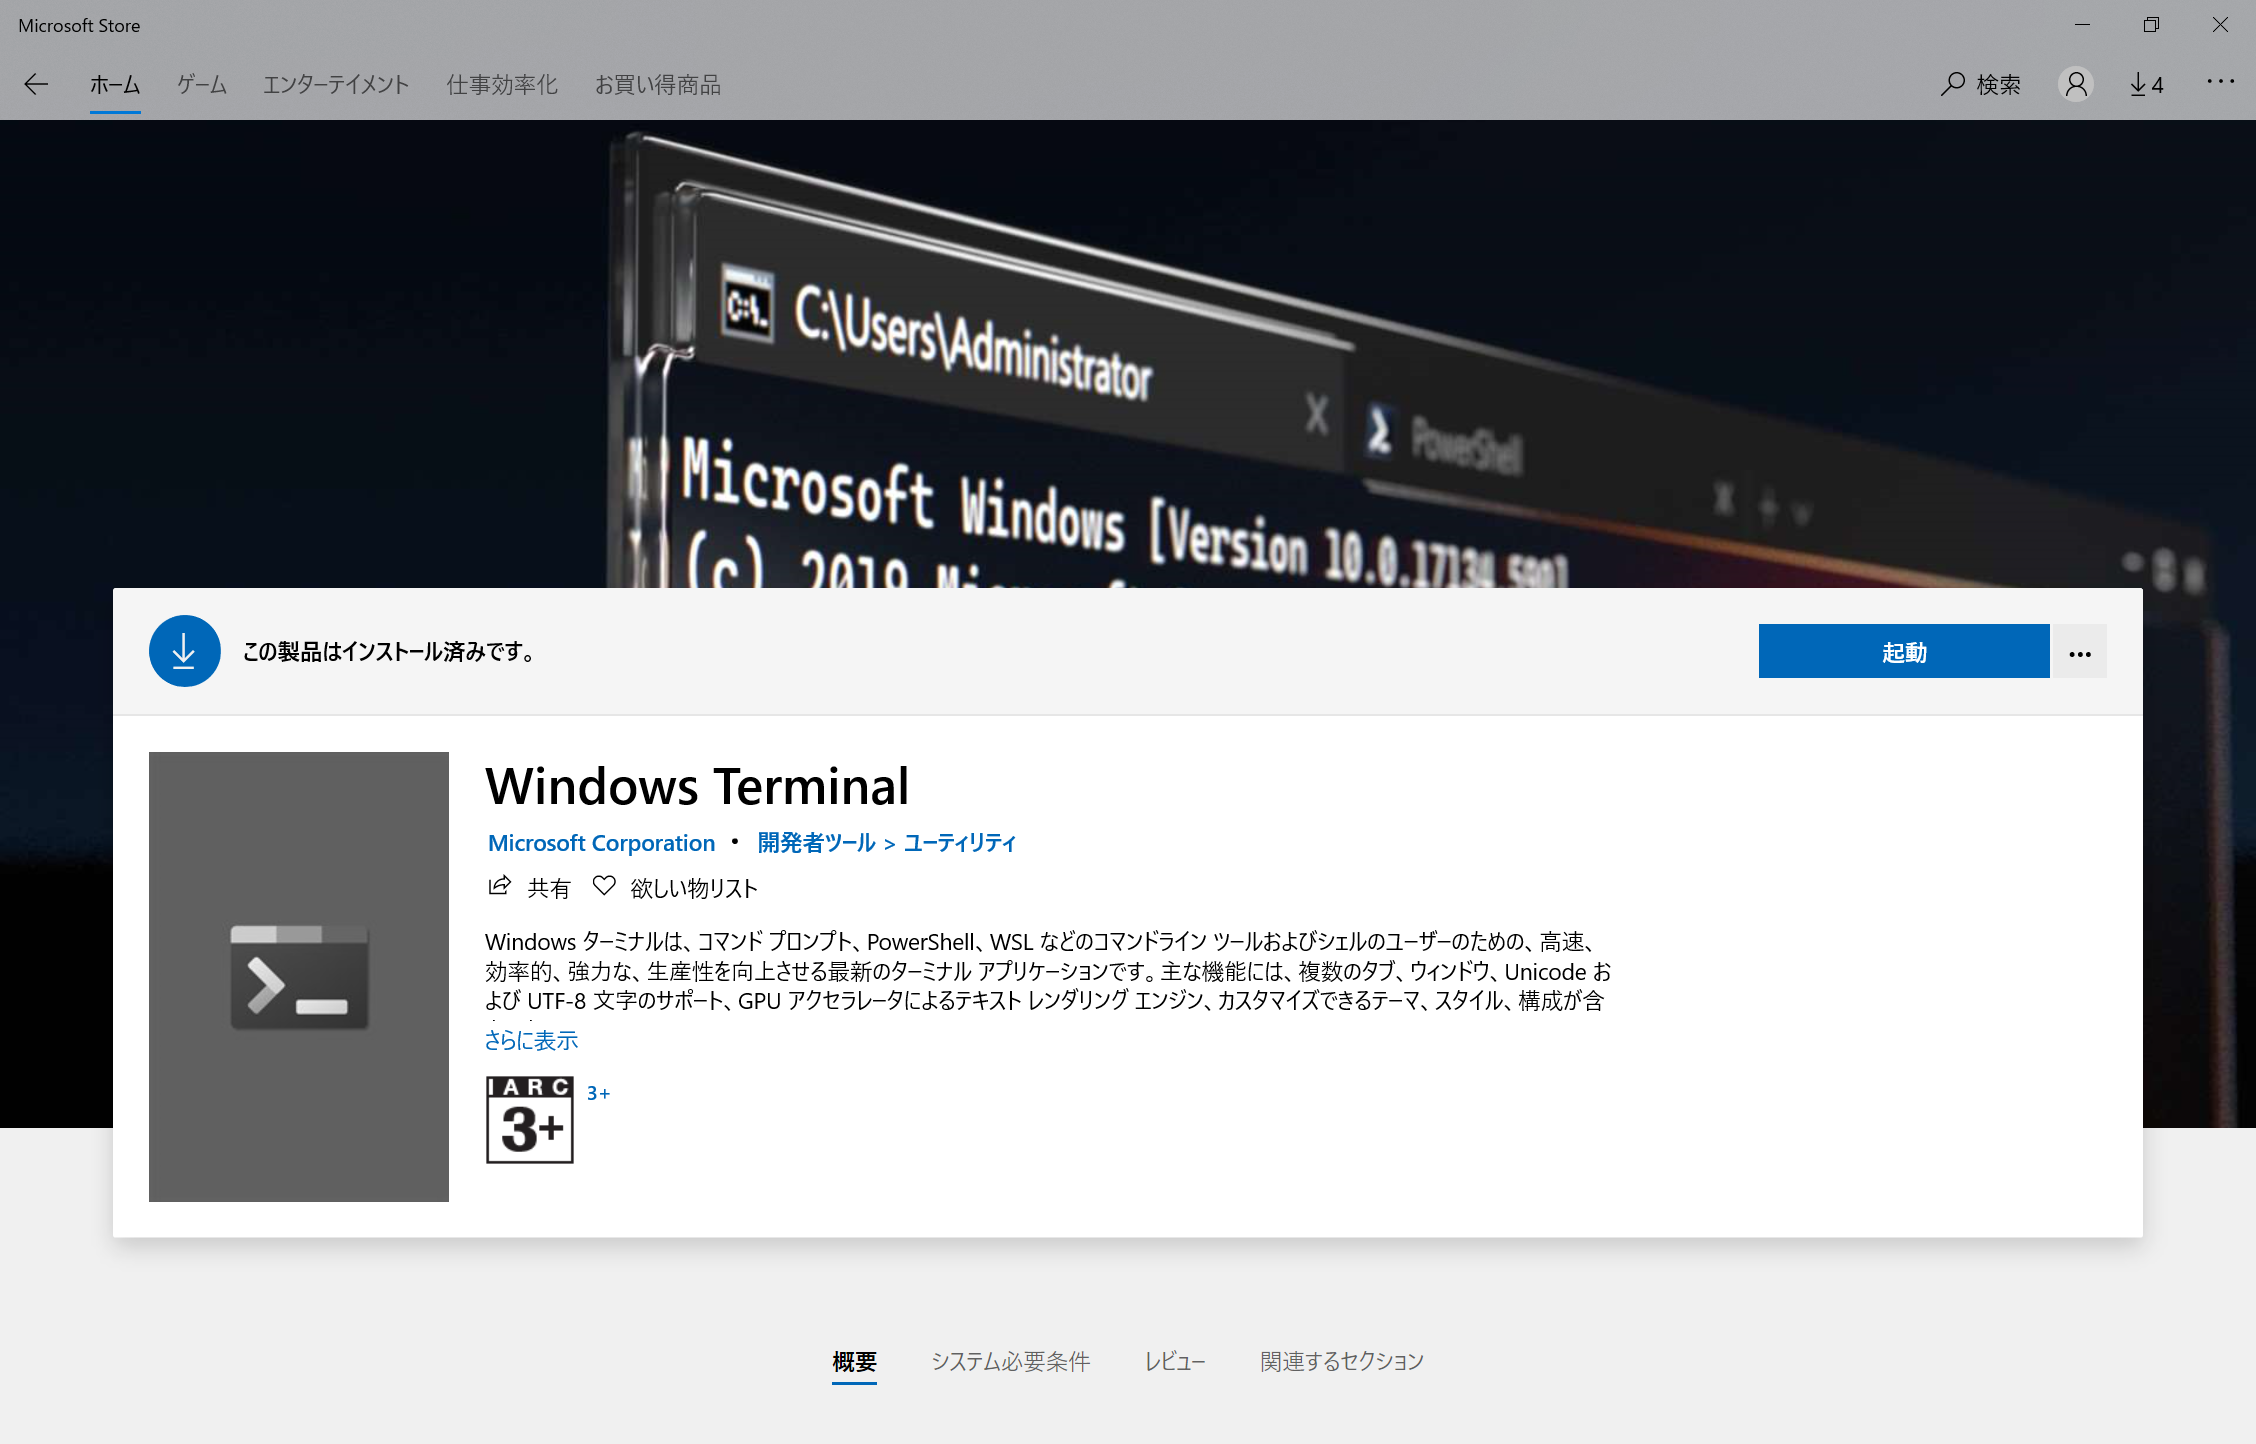
\includegraphics[width=0.5\textwidth]{./fig/install_terminal.png}
        \caption{Windows Terminalのインストール}
        \label{fig:install_terminal}
    \end{figure}
    \item PDFの場合
    \begin{figure}[H]
        \centering
        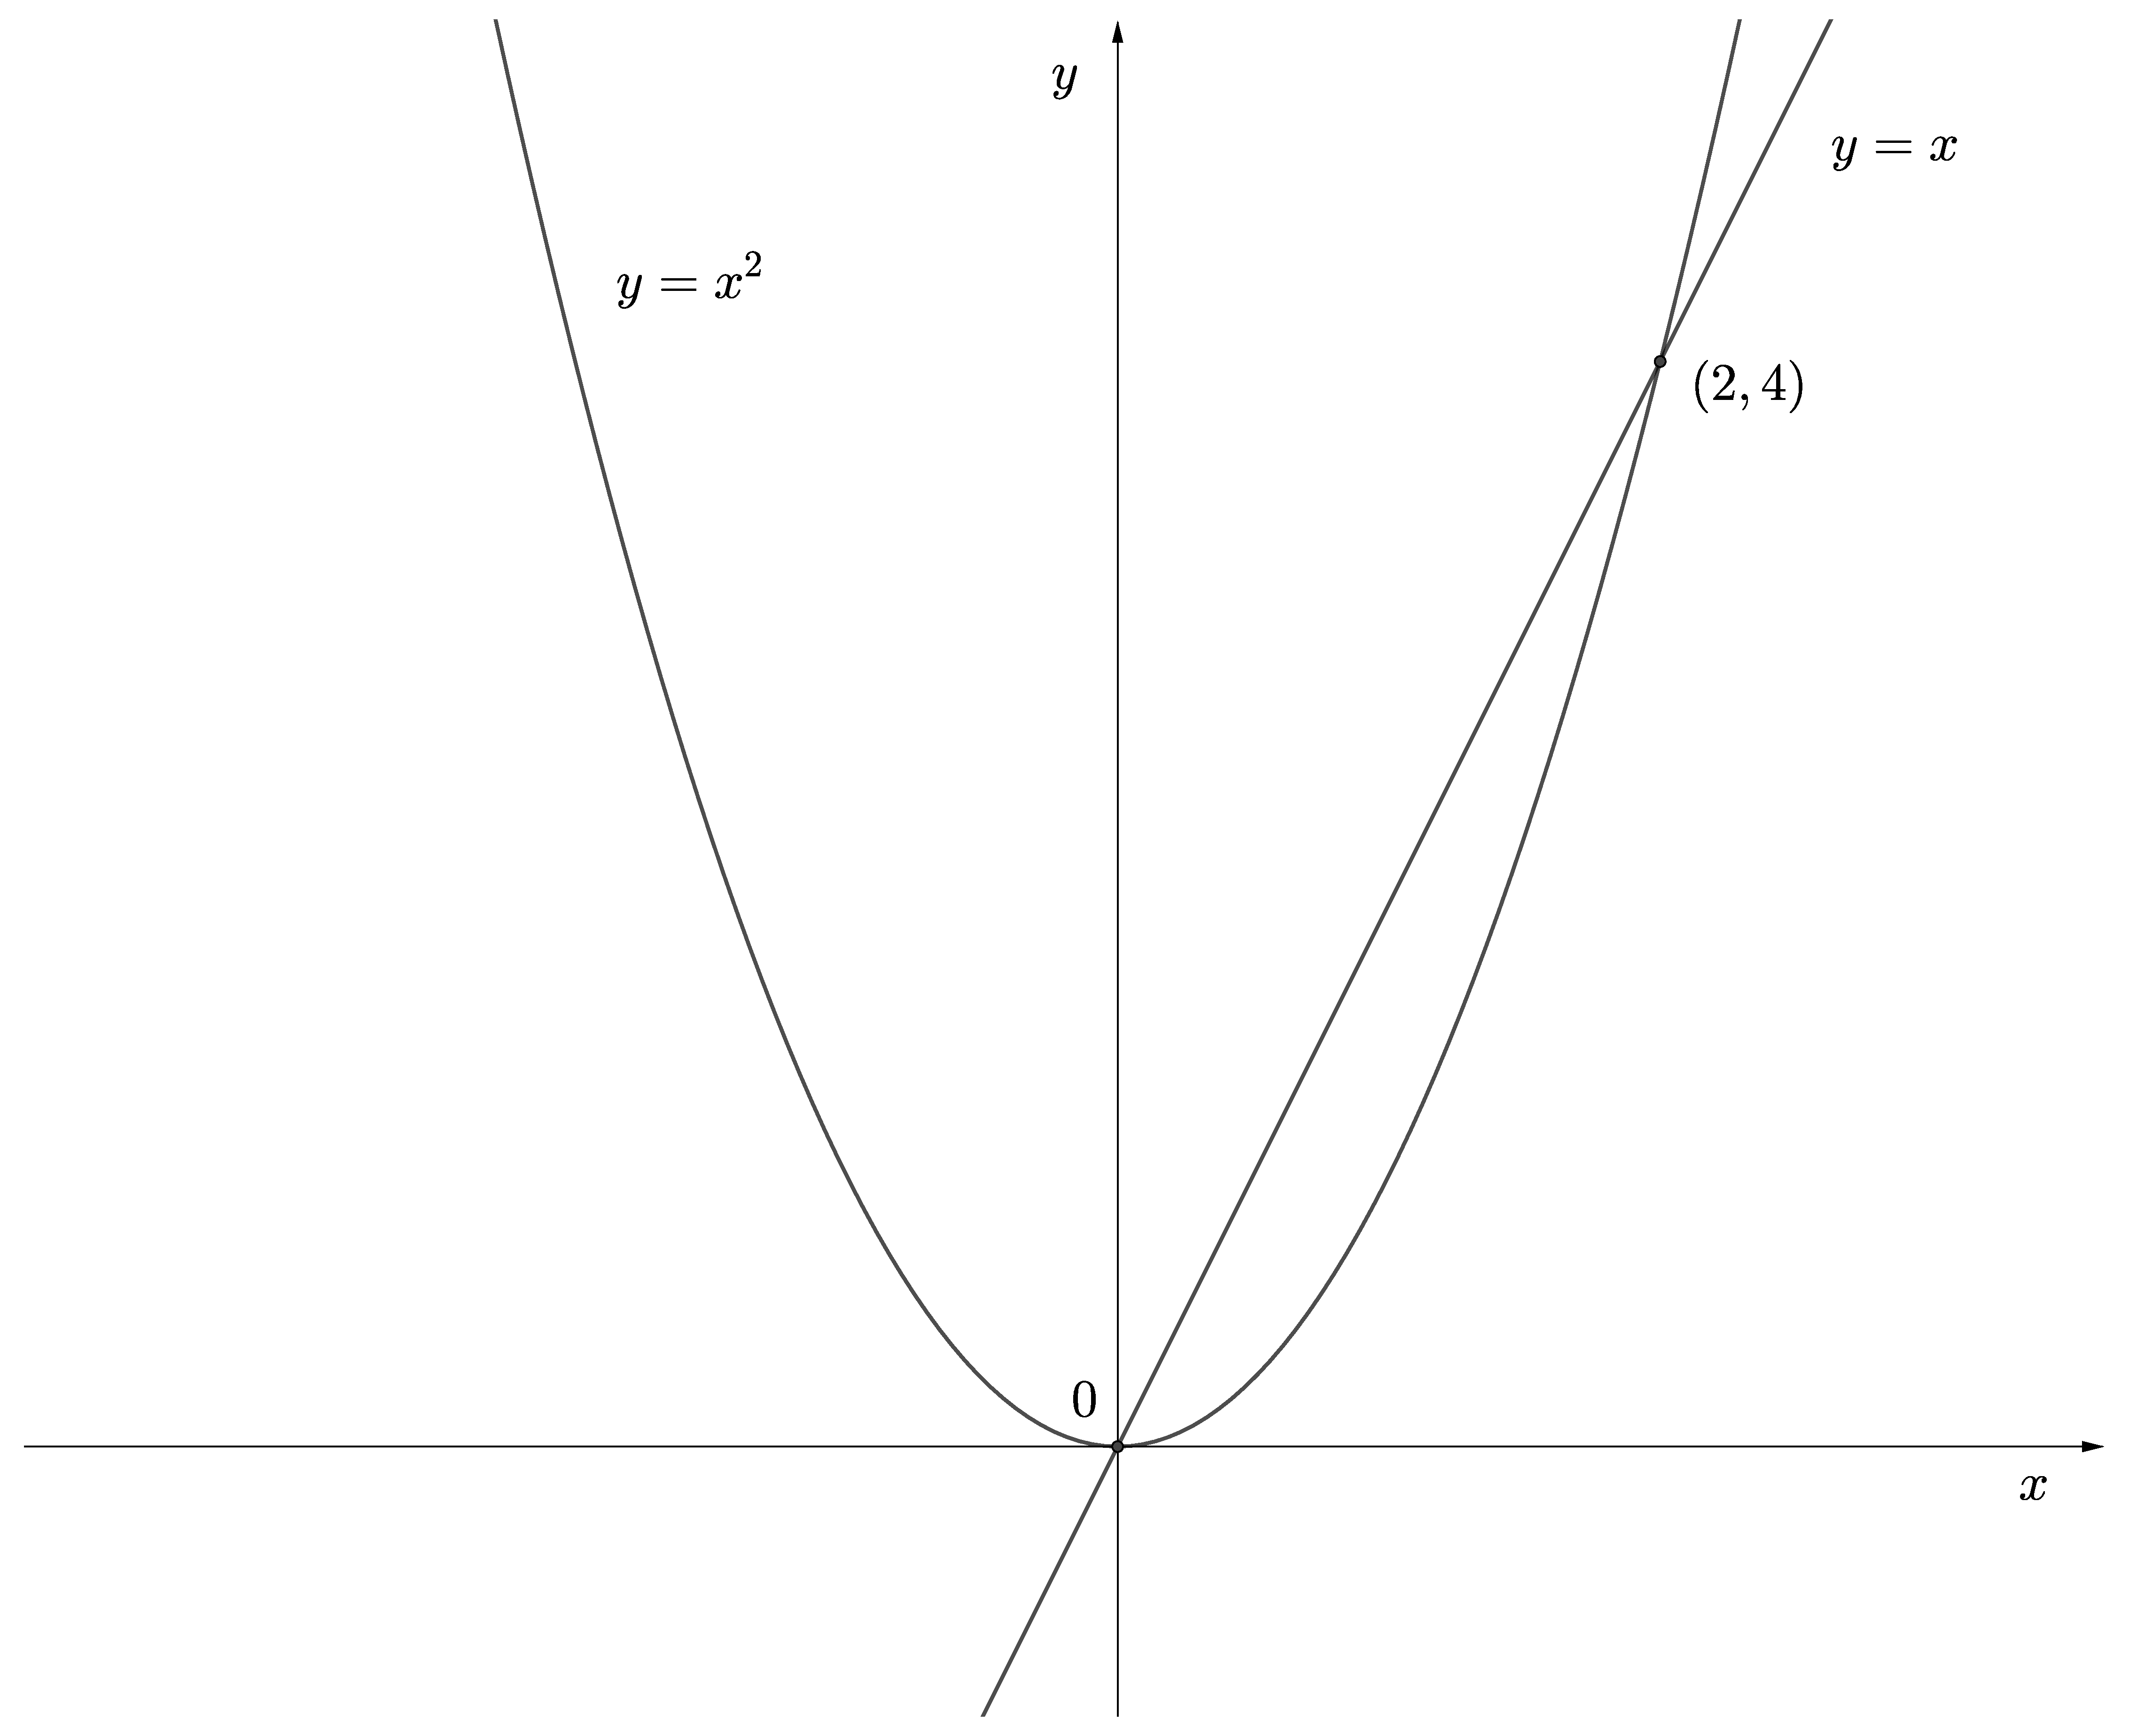
\includegraphics[width=0.5\textwidth]{./fig/graph.pdf}
        \caption{$y=x^2$と$y=x$のグラフ}
        \label{fig:graph1}
    \end{figure}
    \newpage
    \item PDFのページごとの場合
    \begin{figure}[H]
        \centering
        \fbox{
            \includegraphics[width=0.75\textwidth, page=3]{./fig/slide.pdf}
        }
    \end{figure}
    
    \noindent
    \mysection{タイトル}

    これでノート形式の資料も作れる.
\end{itemize}

\section{段組み関連}

\verb|multicols|で段組みが可能.

\begin{multicols}{2}
\subsection{テストA}
ああああああああああああああああああああああああああああああああああああああああああああああああああ.
\subsection{テストB}
ああああああああああああああああああああああああああああああああああああああああああああああああああ.
\end{multicols}

\verb|minipage|でページ分割が可能.

\begin{minipage}{0.6\textwidth}
\begin{table}[H]
  \caption{表の作成}
  \label{table:text}
  \centering
  \begin{tabular}{l|crr}
    \hline 
    メニュー & サイズ & 値段 & カロリー \\ \hline 
    牛丼 & 並盛 & 500円 & 600 kcal \\
    牛丼 & 大盛 & 1,000円 & 800 kcal \\
    牛丼 & 特盛 & 1,500円 & 1,000 kcal \\ \hline
    牛皿 & 並盛 & 300円 & 250 kcal \\
    牛皿 & 大盛 & 700円 & 300 kcal \\
    牛皿 & 特盛 & 1,000円 & 350 kcal \\
    \hline
  \end{tabular}
\end{table}
\end{minipage}
\hfill
\begin{minipage}{0.35\textwidth}
    ああああああああああああああああああああああああああああああああああああああああああああああああああ.
\end{minipage}


\end{document}